\documentclass[11pt,oneside]{book}

%%%%%%%%%%%%% Geometry
\usepackage[a4paper,left=2.5cm,right=2.5cm, bottom=2.5cm,top=2.5cm]{geometry}

%%%%%%%%%%%%%%% Les paquets

\usepackage[english]{babel}
\usepackage[palette=MATa]{nexus}
\usepackage{amsmath}
\usepackage{amssymb}
\usepackage{amsthm}
\usepackage{amsfonts}
\usepackage{multirow}
\usepackage{float}
\usepackage{diagbox}
\usepackage{xcolor}
\usepackage{caption}
\usepackage{graphicx}
\usepackage{subfigure}
\graphicspath{{img/}}
\usepackage{paralist}
\usepackage{tikz}
\usepackage{tikz-cd}
\usepackage{urtheorem}
%%%%%%%%%%%%%%%% hyperref
\usepackage{lipsum}
\usepackage[verbose]{hyperref}
\hypersetup{ 
    hidelinks
}
\setlength{\XeTeXLinkMargin}{-1pt}


\begin{document}

\pagestyle{empty}

\definecolor{plop}{HTML}{4D7186}
\begin{textblock}{1}(0,0)
    \noindent\textcolor{plop}{\rule{\paperwidth}{.55\paperheight}}
\end{textblock}


\begin{textblock}{1}(0,.55)
    \noindent\textcolor{black}{\rule{\paperwidth}{.45\paperheight}}
\end{textblock}


\begin{textblock}{1}(.1,.09)
    \noindent{\fontsize{24.88}{2}\selectfont
        \bfseries\textcolor{white}{Algebra}}
\end{textblock}

\begin{textblock}{1}(.1,.15)
    \noindent {\fontsize{24.88}{2}\selectfont
    \bfseries\textcolor{white}{Definitions and Theorems}}
\end{textblock}


\begin{textblock}{1}(.1,.45)
    \noindent {\fontsize{20.74}{2}\selectfont
        \bfseries\textcolor{white}{Assjock}}
\end{textblock}



\begin{textblock}{.9}(.05,.56)
    \begin{flushright}
        \noindent {\fontsize{20.74}{2}\selectfont
            \bfseries\textcolor{orange}{version 1.1+$\varepsilon$}}
    \end{flushright}
\end{textblock}


\begin{textblock}{.45}(.5,.82)
    \begin{center}
        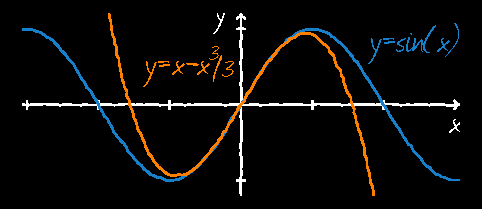
\includegraphics[width=.45\paperwidth]{dlsin}
    \end{center}
\end{textblock}

\begin{textblock}{.4}(.05,.65)
    \begin{center}
        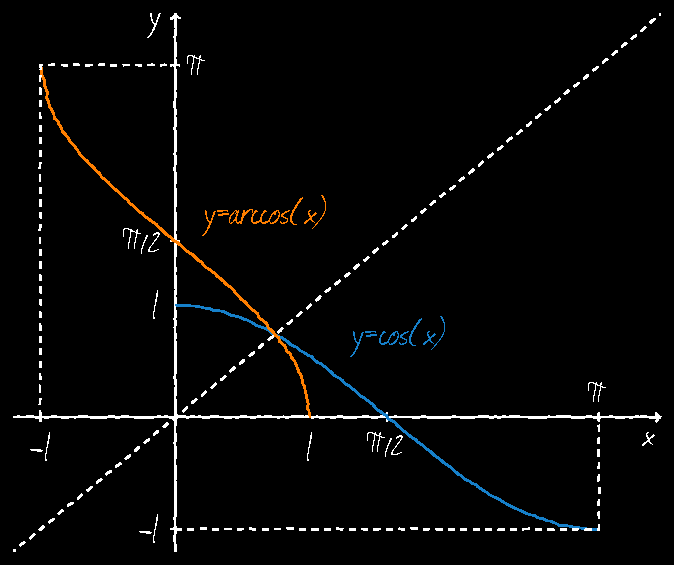
\includegraphics[width=.4\paperwidth]{arccos}
    \end{center}
\end{textblock}


\begin{textblock}{.6}(.05,.6)
    \noindent {\fontsize{20.74}{18}%
    \textcolor{white}{$\displaystyle(a+b)^n = \sum_{k=0}^n 
                \binom{n}{k} a^kb^{n-k}$}}
\end{textblock}


\begin{textblock}{.4}(.4,.77)
    \noindent {\fontsize{17.28}{18}%
    \textcolor{white!80}{$\displaystyle 
                \neg (p\vee q) \equiv (\neg p)\wedge (\neg q)$}}
\end{textblock}

\begin{textblock}{.4}(.1,.93)
    \noindent {\fontsize{14.4}{18}%
    \textcolor{white!50}{$\displaystyle 
                \binom{n}{k} = \frac{n!}{k!(n-k)!}$}}
\end{textblock}


\begin{textblock}{.6}(.5,.69)
    \noindent {\fontsize{17.28}{18}%
    \textcolor{white!10}{$\displaystyle 
                \zeta_k = |a|^{1/n} \mathrm{e}^{i(\mathrm{arg}(a)+2k\pi)/n}$}}
\end{textblock}


\begin{textblock}{.3}(.75,.73)
    \noindent {\fontsize{17.28}{18}%
    \textcolor{white!10}{$\displaystyle \mathrm{e}^{i\pi}+1=0$}}
\end{textblock}



\null\newpage\pagestyle{nexus}

%\tableofcontents
\chapter{Groups}
\section{Logical Symbols}
The logical symbols are a kind of symbols using for theoretical statements.
    \begin{table}[H]
        \centering
        \caption{Frequently-used Logical Symbols}
        \begin{tabular}{|c|c|}\hline
            Symbols&Meanings\\\hline
            $L\Longrightarrow P$& Proposition $L$ is contained in proposition $P$\\
            $L \Longleftrightarrow P $&Proposition $L$ is equivalent to proposition $P$\\
            $\lnot P$&Not $P$\\
            $L\wedge P$&Proposition $L$ and proposition $P$\\
            $L \vee P$&Proposition $L$ or proposition $P$\\
            \hline
        \end{tabular}
    \end{table}
e.g.\[((A\Longrightarrow B)\wedge(\lnot B)\Longrightarrow (\lnot A) )\]


stands for `` if $A$ is contained in  $B$,and $B$ is not true,then $A$ is not true''.

We also call $ A \Longleftrightarrow B$ ``$A$ is the necessary and suffiecent condition of $B$''.

The typical math proposition is like ``$A\Longrightarrow B$''.In order to prove this proposition ,we can use the  implication relationship \[A\Longrightarrow C_1\Longrightarrow \cdots \Longrightarrow C_n\Longrightarrow B\]The every implication relationship in this chain is general truth or proved proposition.

\begin{table}[H]
    \centering
    \caption{Truth Table}
    \begin{tabular}{|c|c|c|c|}
        \hline
        \multirow{2}{*}{$\lnot A$}                       & $A$                    & 0         & 1             \\ \cline{2-4} 
                                                 & $\lnot A$            & 1            & 0             \\ \hline
        \multirow{3}{*}{$A \vee B$}                       &       \diagbox{$A$}{$B$}     &    0        &       1        \\ \cline{2-4} 
                                                 &          0       &   0         &        1        \\ \cline{2-4} 
                                                 &       1         &  1        &        1       \\ \hline
        \multirow{3}{*}{$A \wedge B$}                       &        \diagbox{$A$}{$B$}    &           0&        1          \\ \cline{2-4} 
                                                 &     0         &     0          &      0          \\ \cline{2-4} 
                                                 &        1        &                0       &    1       \\ \hline
        \multirow{3}{*}{$A\Longrightarrow B$}                      &  \diagbox{$A$}{$B$} & 0  &  1 \\ \cline{2-4} 
                                                & 0  &  1 &  1 \\ \cline{2-4} 
                                                & 1  &  0 & 1  \\ \hline
        \end{tabular}
    \end{table}
\begin{question}$\lnot (A\wedge B )\Leftrightarrow (\lnot A \vee \lnot B)$.
\end{question}
\begin{proof}
    (Use the truth table)

    If $A$ is ture, $B$ is ture, $A\wedge B$ is ture. $\lnot (A\wedge B)$ is false.$\lnot A $ is false,$\lnot B$ is false, $(\lnot A \vee \lnot B)$ is false.

    If $A$ is ture, $B$ is false, $A\wedge B$ is false. $\lnot (A\wedge B)$ is true.$\lnot A $ is false,$\lnot B$ is true, $(\lnot A \vee \lnot B)$ is ture.

    If $A$ is flase, $B$ is true, $A\wedge B$ is false. $\lnot (A\wedge B)$ is true.$\lnot A $ is true,$\lnot B$ is false, $(\lnot A \vee \lnot B)$ is ture.

    If $A$ is false, $B$ is false, $A\wedge B$ is false. $\lnot (A\wedge B)$ is true.$\lnot A $ is true,$\lnot B$ is true, $(\lnot A \vee \lnot B)$ is ture.

    So
    \[\lnot (A\wedge B )\Leftrightarrow (\lnot A \vee \lnot B)\]
\end{proof}    

\begin{question}
    $(A \Rightarrow B)\Leftrightarrow\lnot A \vee B$.
\end{question}
\begin{proof}
    Firstly, we confirm the truth of \[(A \Rightarrow B)\Rightarrow\lnot A \vee B\]

    If $(A \Rightarrow B)$ is false, then $\lnot A \vee B$ is true.

    If $(A \Rightarrow B)$ is ture ,then we have two posibilities. The first is $A$ is ture, $B$ is true, so $\lnot A \vee B$ is true. The second is $A$ is false,then $B$ can be true or false, but $\lnot A \vee B$ will be true.

    Hence, $(A \Rightarrow B)\Rightarrow\lnot A \vee B$.

    Secondly, we prove \[(A \Rightarrow B)\Leftarrow\lnot A \vee B\]

    If $\lnot A \vee B$ is false, then $(A \Rightarrow B)$ is true.

    If $\lnot A \vee B$ is true, we have
    \begin{enumerate}
        \item $\lnot A$ is true, $B$ is false, then, $A$ is false, $(A \Rightarrow B)$ is true.
        \item $\lnot A$ is false, $B$ is true, then, $A$ is true, $(A \Rightarrow B)$ is true.
        \item $\lnot A$ is true, $B$ is true, then, $A$ is false, $(A \Rightarrow B)$ is true.
    \end{enumerate}

    So $(A \Rightarrow B)\Leftarrow\lnot A \vee B$.
\end{proof}



\end{document}